\section{Referencial Teórico}
Nesta seção, serão apresentados os conceitos e ferramentas utilizados neste trabalho, através de uma revisão da literatura a fim assegurar a compreensão por completo do projeto. 

\subsection{\textit{CAPTCHA}}

Desenvolvido em meados de 1997 para o site Alta Vista e, posteriormente para o \textit{Yahoo}, o \textit{Captcha} (\textit{Completely Automated Public Turing test to tell Computers and Humans Apart}. Na tradução: Teste de \textit{Turing} público completamente automatizado para diferenciação entre computadores e humanos) é utilizado como uma ferramenta de segurança anti-spam cuja premissa é utilizar uma mensagem distorcida como desafio para comprovar que o acessante é um ser humano, em vez de um robô / computador.

O Teste de Turing (postulado por  Alan Turing, em 1950) é uma forma de determinar se as atividades de máquina inteligentes podem ser assimiladas ao comportamento humano.  Qualquer sistema (incluindo o CAPTCHA) se converge em gerar questões nas quais apenas seres humanos e não os computadores, por mais inteligentes que sejam, não conseguiriam resolver. No caso do CAPTCHA, a pergunta desafio pode ser de referência à interpretação de mensagens alfanuméricas distorcidas em imagens, interpretação de objetos e cliques em partes específicas de uma imagem; partindo da premissa de que máquinas com inteligência artificial, por mais aperfeiçoadas que sejam, não conseguiriam interpretar de forma razoável.

\subsection{Aprendizado de Máquina}

Atualmente a produção de dados (imagens, textos, sons, vídeos, dentre outras fontes) está em crescimento. A maior distinção neste cenário é que as informações criadas/processadas ao redor do globo não são produzidas apenas por seres humanos, mas sim, dispositivos eletrônicos e aplicações. 

Devido a imensa quantidade de dados gerados, os seres humanos, incapacitados de interpretar tamanhas quantidades, terceirizam cada vez mais esta função para dispositivos dotados de inteligência artificial através do conceito de aprendizado de máquina que, por sua vez, utiliza-se de ferramentas e tecnologia que buscam responder perguntas e gerar \textit{insights} através do consumo dados\cite{santos2018identificaccao}.

O aprendizado de máquina é o campo de estudo que dá aos computadores a capacidade de aprender sem serem explicitamente programados. Utiliza-se de algoritmos que podem compreender e assimilar seus erros e tecer previsões a partir de amostras de dados, ou tomar decisões guiadas unicamente pelos mesmos. O aprendizado de máquina é aplicado em tarefas computacionais onde criação e programação de algoritmos torna-se inviável \cite{russell2002artificial}.

\subsubsection{Treinamento para Aprendizado de Máquina}

A premissa básica para todo aprendizado de máquina é o "treinamento" desta onde se usa dados previamente selecionados para criação e parametrização do determinado modelo de predição, que é usado para gerar previsões de resultados futuros de acordo com os estímulos que o agente inteligente receber \cite{russell2002artificial}. Contudo, para que o próprio treinamento seja satisfatório, os dados devem ser tratados previamente de modo a selecionar quais dados são importantes de fato para o aprendizado. Fato este que requer muito esforço \cite{russell2002artificial}.

\subsubsection{Aplicações do Aprendizado de Máquina}

A utilização de aprendizado de máquina é amplamente ut paira suas aplicilzações a fim de personalizar os seus produtos de forma automatizada para cada usuário, como em recomendação de vídeos, identificação fácil, sistemas de saúde, segurança, entre outras aplicações. Há três grandes categorias de aprendizado de máquina: supervisionado, não-supervisionado e reforço \cite{russell2002artificial}. Aqui, foi usado o aprendizado supervisionado, portanto esse será o foco.

\subsubsection{Aprendizado Supervisionado}

Neste tipo de aprendizado, os dados são rotulados, então eles são corretos para realizar o treinamento do modelo. Esse método é deveras eficiente, já que o sistema pode trabalhar com informações corretas \cite{russell2002artificial}. 

A rotulação dos dados é o cerne deste tipo de aprendizado, pois quando os rótulos são contínuos, então o problema é de regressão e quando forem discretos, então o problema é de classificação \cite{russell2002artificial}.

Vejamos dois exemplos:
\begin{enumerate}
    \item Regressão — Dada uma imagem de homem/mulher, tentar prever sua idade com base em dados da imagem.
    \item Classificação — Dada um exemplo de tumor cancerígeno, tentar prever se ele é benigno ou maligno através do seu tamanho e idade do paciente.
\end{enumerate}

Em resumo, o aprendizado supervisionado realiza um treinamento de um modelo por meio de um histórico de dados rotulados e realiza predições de outros dados futuros não rotulados \cite{santos2018identificaccao}, onde no primeiro exemplo seria a imagem de homem/mulher e no segundo exemplo as características de um tumor.

É aplicável quando o sistema já entende quais entradas estão associadas com determinadas saídas e deve aprender um método de montar essa associação. Usam a compreensão de padrões para tecer previsões \cite{russell2002artificial}.

%\subsection{Redes Neurais Artificiais (RNA)}
\subsection{Visão Computacional}

Visão Computacional é a capacidade responsável pela visão de uma máquina, pela maneira como o computador vislumbra o ambiente à sua volta, angariando informações advindas de imagens capturadas por diversos dispositivos \cite{de2014visao}. Isso permite o reconhecimento, manipulação e pensamento sobre objetos que compõem uma imagem.

Os olhos humanos são capazes de perceber e entender objetos em uma imagem rapidamente. Isso ocorre no córtex visual do cérebro. Há estudos focados em entender o funcionamento dessa parte do cérebro, e trazer isso para o conceito de visão computacional, no que se refere à ``ensinar computadores a enxergarem como humanos'' \cite{david1962eyes}.

Sistemas de visão computacional usualmente são especialistas, ou seja, necessitam de conhecimento específico para solucionar determinado(s) problema(s). Portanto, há muitas formas de se implementar um sistema de visão computacional. De acordo com Milano e Honorato (2014)\nocite{de2014visao}, há, minimamente,uma organização de processos comuns nesses tipos de sistemas, na ordem que se segue:

\begin{enumerate}
    \item Aquisição de Imagem
    \item Pré-processamento:  a aplicar métodos específicos que facilitem a identificação de um objeto.
    \item Extração de características: Extração de características matemáticas que compõem uma imagem.
    \item Detecção e segmentação: Processo realizado para destacar regiões relevantes da imagem.
    \item Processamento de alto nível: Processo que inclui validação da satisfação dos dados obtidos e classificação dos objetos obtidos em diferentes categorias.
\end{enumerate}

\subsection{Redes Neurais Convolucionais (CNN)}
As Redes Neurais Convolucionais (\textit{Convolutional Neural Networks}, CNNs) foram propostas inicialmente em 1998, aonde os autores construíram uma arquitetura de rede neural chamada \textit{LeNet5}, utilizada para reconhecer dígitos escritos à mão \cite{lecun1998gradient}.

As \textit{CNNs} são similares às redes neurais tradicionais, já que em ambos os casos são compostos por neurônios com seus respectivos pesos e bias que requerem treinamento \cite{haykin2007redes}. Cada neurônio é alimentado por algumas entradas. Em seguida é aplicado a ele o produto escalar das entradas e pesos, e uma função não-linear. 

O trunfo das \textit{CNNs} está no tipo de entrada, imagens \cite{santos2018identificaccao}. Isso permite codificar propriedades na arquitetura da rede, distintivamente das redes neurais tradicionais, uma vez que esse último produz um número muito alto de pesos a serem treinados, tornando inviável e não escalável para o tipo de entrada imagem.

\subsubsection{Arquitetura}

A estrutura de uma CNN é composta por uma série de camadas. A primeira camada é a entrada (\textit{input}), usualmente sendo uma imagem com suas características de largura, altura e profundidade. Depois da entrada, vem três camadas próprias da CNN: camada convolucional, camada de \textit{pooling} e camada totalmente conectada. É também comum que exista a camada de ativação logo após a convolução  \cite{haykin2007redes}. A Figura \ref{fig:arch} demonstra a arquitetura de forma genérica.

\begin{figure}
    \centering
    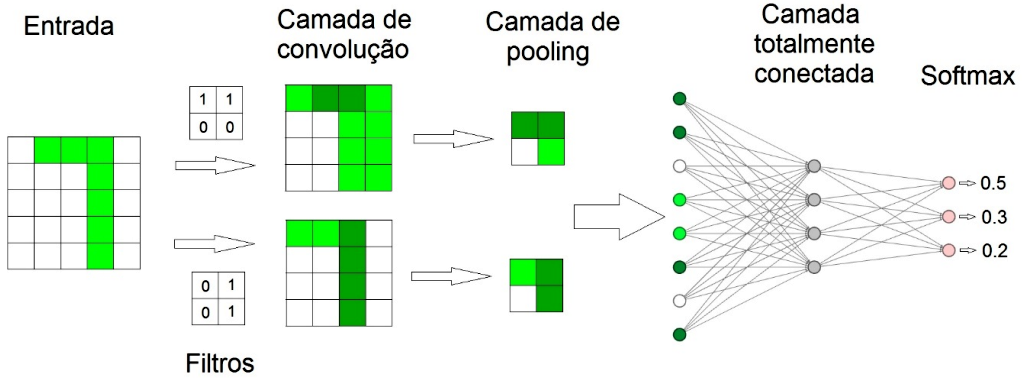
\includegraphics[scale=0.25]{Relatorio/figuras/arch.png}
    \caption{Arquitetura de uma CNN \cite{eliveltoebermamrenatoa.krohling2018}}
    \label{fig:arch}
\end{figure}

As \textit{CNNs} são arquitetadas estritamente para reconhecimento de formas bidimensionais com um alto grau de invariância quanto a translação, escalonamento, inclinação e outras formas de distorção \cite{haykin2007redes}.

\subsubsection{Camada Convolucional}

A camada convolucional efetua a parcela mais pesada do processamento computacional. Nessa camada, cada neurônio não está ligado a todas as entradas da rede. Além disso, a camada é composta por um conjunto de filtros, que são pequenas matrizes de valores reais capazes de aprender de acordo com o treinamento. Por falar em treinamento dos filtros, nesse momento há operações de convolução para reconhecer a imagem de entrada e criar um mapeamento de características. Isso significa que, se o conjunto de valores de um filtro for capaz de retratar uma região da imagem, a rede como um todo compreende que estes mesmos valores poderão ser usados para identificar outra região da entrada se posto em outro filtro. Mesmo assim, os valores dos filtros variam ao longo do treinamento a fim de tecer reparos, adequações e executar melhores extrações de características de uma imagem de entrada.

\begin{figure}
    \centering
    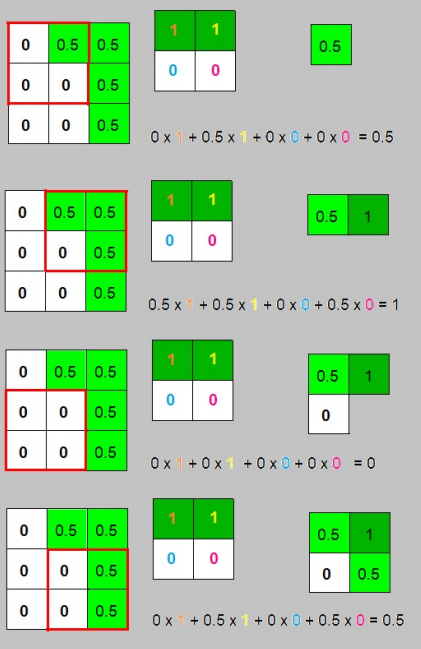
\includegraphics[scale=0.3]{Relatorio/figuras/stride.png}
    \caption{Operação de convolução e \textit{strides} em matrizes de entrada \cite{eliveltoebermamrenatoa.krohling2018}}
    \label{fig:stride}
\end{figure}

A Figura \ref{fig:stride} demonstra um fenômeno de deslizamento de quadro que seleciona uma quantidade de valores. Isso é orientado pelo parâmetro \textit{stride}. Na figura, o filtro desloca-se pela imagem 1 pixel por vez para os lados e para baixo. Às vezes o tamanho do filtro e do \textit{stride} não se adequam a imagem, tendo então que acionar o \textit{zero-padding}. Isso não é nada mais do que colocar zeros na borda da imagem para que o deslizamento ocorra \cite{haykin2007redes}.

A camada convolucional emprega muitos neurônios para esquematizar a entrada, mas em uma quantidade fixada. Por limitar a quantidade de neurônios, o número de conexões diminui, entretanto facilita a otimização dos parâmetros internos, os quais tornam-se mais importantes.

\subsubsection{Camada de \textit{Pooling}}

A camada de \textit{pooling}, em resumo, simplifica o resultado da camada antecessora. Da mesma forma que na convolução, é escolhida uma unidade de área para transitar por toda saída da camada anterior. Isso serve para resumir a informação de determinada área em um valor apenas (Figura \ref{fig:pooling}). Por exemplo, se a saída da camada anterior for 24x24 e a unidade de área definida for 2x2, então a saída do \textit{pooling} é uma matriz 12x12. Não basta apenas transitar, mas saber como será a sua sumarização. O meio mais empregado para isso é o \textit{maxpooling}, aonde apenas o maior número da unidade é enviado à saída. Isso serve para decrescer a quantidade de pesos a serem aprendidos e também evitar o \textit{overfitting}.

\begin{figure}
    \centering
    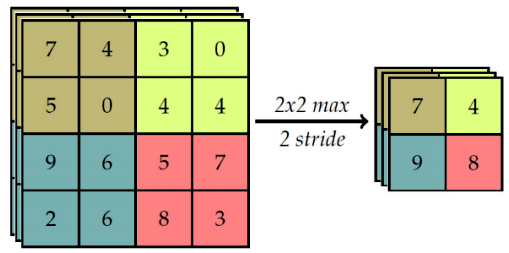
\includegraphics[scale=0.3]{Relatorio/figuras/pooling.png}
    \caption{\textit{Pooling} com \textit{maxpooling} \cite{santos2018identificaccao}}
    \label{fig:pooling}
\end{figure}


\subsubsection{Camada Totalmente Conectada}

Essa camada se caracteriza pela completude de conexões com a camada antecessora, onde sua entrada é a saída da camada anterior e sua saída são N neurônios, com N sendo a quantidade de classes do modelo para finalizar a classificação (Figura  \ref{fig:full}). É a última camada de uma CNN, já que atua do mesmo modo que as redes neurais tradicionais. É possível então adicionar as mesmas técnicas de melhoramento de desempenho da camada, como o \textit{dropout}, por exemplo \cite{eliveltoebermamrenatoa.krohling2018}.

\begin{figure}
    \centering
    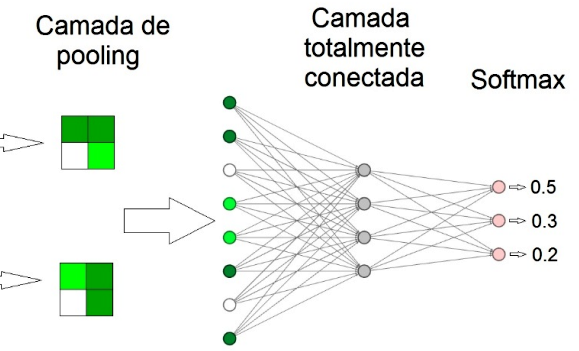
\includegraphics[scale=0.3]{Relatorio/figuras/full_conected.png}
    \caption{Camada totalmente conectada, com \textit{softmax} \cite{eliveltoebermamrenatoa.krohling2018}}
    \label{fig:full}
\end{figure}

Na saída (elemento mais ao extremo) é aplicada a função \textit{softmax} para se ter a probabilidade de dada entrada pertencer a uma certa classe (Figura \ref{fig:full}). Aqui é realizado o algoritmo de treinamento supervisionado \textit{backpropagation}. O erro obtido nesta camada é propagado para que os pesos dos filtros das camadas convolucionais sejam ajustados. Assim, os valores dos pesos compartilhados são aprendidos ao longo do treinamento.


\subsection{Funções de Ativação}

Funções de ativação basicamente decidem se um neurônio deve ser ativado, ou não. É a transformação não-linear que é feita ao longo do sinal de entrada. De modo simplificado, o funcionamento de um neurônio artificial baseia-se em tecer um cálculo, que é a soma ponderada das entradas com um bias, para decidir sobre seu disparo \cite{santos2018identificaccao}. Esta saída é então encaminhada como entrada para a próxima camada de neurônios. A função de ativação faz a transformação não-linear dos dados de entrada, sendo possível então a rede aprender a executar tarefas mais complexas (Processamento de linguagem natural, Visão computacional etc) \cite{haykin2007redes}. A equação abaixo resume esse cálculo feito:
\begin{center}
$w\ast x + b = y$    
\end{center}
Na equação, \textit{x} é o conjunto de  entradas, \textit{w} os pesos, \textit{b} é o \textit{bias} (elemento que usado para aumentar o grau de liberdade dos ajustes dos pesos \cite{haykin2007redes}) e \textit{y} é a pontuação para cada classe.

\subsubsection{Função Unidade Linear Retificada (ReLU) \cite{russell2002artificial}}

A função de ativação ReLU resolve \textit{f(x) = max(0,x)}, portanto a ativação se dá por um limiar em zero. De acordo com Santos et al. (2018) \nocite{santos2018identificaccao}, as caraterísticas dessa função são:

\begin{itemize}
    \item Acelera a convergência do Gradiente descendente quando se compara às funções \textit{sigmoid} e \textit{tanh}.
    \item É implementada com funções menos custosas que a sigmoide e a \textit{tanh}.
    \item Pode inativar neurônios quando a soma ponderada de todas as entradas são negativas. \textit{ReLU} não propaga erro no \textit{backpropagation}, nesses casos.
    \item A relação de recorrência que define o \textit{ReLU} é dado por:
    \begin{equation}
        f(x)=\begin{cases}
        0, & \text{se $x<0$}.\\
        x, & \text{senão}
        \end{cases}
    \end{equation}
\end{itemize}

\subsubsection{Função \textit{SoftMax}}

De acordo com Ebermam e Krohling (2018), essa função é aplicada em redes neurais de classificação, sendo a última camada e responsável por apresentar resultados . Essa função estimula a saída da rede a representar a chance dos dados serem de uma determinada classe. É muito útil quando tem que se lidar com várias classes. Essa função transforma as saídas para cada classe em valores entre 0 e 1 e também divide pela soma das saídas. Isso essencialmente dá a probabilidade de a entrada estar em uma determinada classe. A quantidade de neurônios nela é definido pelo número de classes do problema. Pode ser definida pela equação:

\begin{center}
$y_{j} = \frac{e^{y(j)}}{\sum_{i=1^{e^{y(i)}}}^{n}}$
    
\end{center}

A saída \textit{y} do neurônio \textit{j} passa a ser o valor da mesma dividido pelo somatório de todas as saídas dos neurônios dessa camada. 

\subsection{Função de otimização Adam}

De acordo com Kingma e Ba (2014)\nocite{kingma2014adam}, o Adam é um meio para otimização estocástica eficiente que requer gradientes de primeira ordem com pouco consumo de memória. Esse método calcula as taxas de aprendizagem para diferentes parâmetros a partir de estimativas do primeiro e segundo \textit{momentum} dos gradientes.
Por sua vez, \textit{Momentum} \cite{santos2018identificaccao} é um termo na função de otimização que assume um valor entre 0 e 1 e tem como finalidade aumentar o tamanho das iterações que buscam o mínimo erro. Se o valor do \textit{momentum} for grande, a taxa de aprendizado deverá ser mantida menor.

\subsection{\textit{Overfitting}}

\textit{Overfitting} é quando a diferença entre o valor de perda para o conjunto de treinamento e o valor de perda do conjunto de teste é muito grande \cite{santos2018identificaccao}. Isso quer dizer que, é notável que a rede memoriza os padrões do treinamento, mas não consegue generalizar, não podendo então prever as saídas corretamente.

\subsection{Dropout}

\textit{Dropout} é a remoção aleatória de neurônios no processo de aprendizagem, a fim de se evitar o \textit{overfitting}. Em outras palavras, ele elimina neurônios individuais a cada etapa do treinamento, tornando a rede neural mais reduzida, com menos conexões e parâmetros, com o objetivo final de melhorar o desempenho da rede.

\subsection{Matriz de Confusão}
De acordo com Souza (2019)\nocite{souza_2019}, matriz de confusão é uma tabela que mostra as frequências de classificação para cada classe do modelo. Ela vai nos mostrar as frequências:
\begin{itemize}
    \item Verdadeiro positivo (\textit{true positive — TP}): ocorre quando no conjunto real, a classe que estamos buscando foi prevista corretamente.
    \item Falso positivo (\textit{false positive — FP}): ocorre quando no conjunto real, a classe que estamos buscando prever foi prevista incorretamente. 
    \item Falso verdadeiro (\textit{true negative — TN}): ocorre quando no conjunto real, a classe que não estamos buscando prever foi prevista corretamente.
    \item Falso negativo (\textit{false negative — FN}): ocorre quando no conjunto real, a classe que não estamos buscando prever foi prevista incorretamente.

\end{itemize}

As matrizes de confusão são inerentemente conectadas aos seguintes conceitos:

\begin{itemize}
    \item Acurácia: Diz quanto o meu modelo acertou das previsões possíveis. E a razão entre o somatório das previsões corretas sobre o somatório das previsões:
    \begin{center}
        $acurácia = \frac{TP+TN}{TP+FP+TN+FN} = \frac{predições corretas}{total das predições}$
    \end{center}
    \item Recall: O quão bom o modelo é para prever positivos, sendo positivo entendido como a classe que se quer prever. É definido como a razão entre verdadeiros positivos sobre a soma de verdadeiros positivos com negativos falsos:
    \begin{center}
        $recall = \frac{TP}{TP+FN}$
    \end{center}
    \item Precisão: a proporção de identificações positivas:
    \begin{center}
        $precisao = \frac{TP}{TP+FP}$
    \end{center}
    \item f-score: o balanço entre a precisão e o recall de nosso modelo:
    \begin{center}
        $f-score = 2*\frac{precisao*recall}{precisao+recall}$
    \end{center}
\end{itemize}

\subsection{Ferramentas}

\subsubsection{\textit{Tensorflow}}

\textit{TensorFlow} é uma biblioteca de software de código aberto para computação numérica usando grafos computacionais. Foi originalmente desenvolvido pela \textit{Google Brain Team} na organização de pesquisa \textit{Machine Intelligence} do \textit{Google} para aprendizado de máquina e pesquisa de redes neurais profundas (\textit{Deep Learning}), mas a biblioteca é geral o suficiente para ser aplicada em uma grande variedade de outros domínios também. Foi disponibilizado como \textit{open-source} em 2015 e alcançou a versão 1.0 em Fevereiro de 2017, com um desenvolvimento e adoção incrivelmente rápidos e muitos colaboradores externos. O \textit{TensorFlow} vem se tornando a biblioteca padrão para desenvolvimento em \textit{Deep Learning} e aplicações de Inteligência Artificial. Este artigo apresenta o \textit{TensorFlow}, sua comunidade e ecossistema de software livre. Afinal, O Que é o \textit{TensorFlow Machine Intelligence Platform}?

A versão \textit{open-source} do \textit{TensorFlow} foi liberada pelo Google em Novembro de 2015, como o resultado de anos de lições aprendidas do seu antecessor, o \textit{DistBielief}. O \textit{TensorFlow} foi construído para ser flexível, eficiente, extensível e portável. Computadores de qualquer natureza podem executar o \textit{TensorFlow}, desde \textit{smartphones} a gigantescos \textit{clusters} de computadores. E uma das características mais interessantes do \textit{TensorFlow} é sua capacidade de rapidamente gerar um produto ou serviço a partir do modelo preditivo treinado, eliminando a necessidade de reimplementar o modelo. O \textit{TensorFlow} é uma biblioteca inovadora e conta com uma comunidade ativa. O \textit{TensorFlow} pode ser usado por indivíduos em busca de pesquisas ou mesmo grandes empresas que precisam implementar estratégias de Inteligência Artificial. O \textit{Google} é um claro exemplo.

A ferramenta original de \textit{Deep Learning} em larga escala do \textit{Google} era o \textit{DistBelief}, um produto da equipe do \textit{Google Brain}. Desde a sua criação, tem sido utilizado por dezenas de equipes para inúmeros projetos envolvendo redes neurais profundas. No entanto, como ocorre com muitos projetos de engenharia de primeira classe, houve erros de projeto que limitaram a usabilidade e a flexibilidade do \textit{DistBelief}. Algum tempo após a criação do \textit{DistBelief}, o \textit{Google} começou a trabalhar no seu sucessor, cujo design aplicaria lições aprendidas com o uso e as limitações do \textit{DistBelief} original. Este projeto transformou-se no \textit{TensorFlow}, que rapidamente se tornou uma biblioteca popular para o aprendizado de máquina e está sendo usado atualmente para aplicações de Inteligência Artificial, como Processamento de Linguagem Natural, Visão Computacional e análise preditiva.

O \textit{TensorFlow} é multiplataforma e pode ser usado no \textit{Windows, MacOS} e Linux. Ele é executado em quase tudo: \textit{CPUs} e \textit{GPUs} – incluindo plataformas móveis e integradas – e até mesmo \textit{Tensor Processing Units} (\textit{TPUs}), que são hardware especializado para fazer a matemática de um tensor (um objeto matemático multidimensional). O \textit{TensorFlow} é projetado para ser escalável em vários computadores, bem como várias \textit{CPUs} e \textit{GPUs} dentro de máquinas individuais. Embora a implementação de código aberto original não tivesse recursos distribuídos após a liberação, a partir da versão 0.8.0 a funcionalidade de execução distribuída ficou disponível como parte da biblioteca \textit{TensorFlow}. Embora esta \textit{API} (\textit{Application Programming Interface}) distribuída seja um pouco pesada, é incrivelmente poderosa. A maioria das outras bibliotecas de aprendizagem de máquina não possui esses recursos e é importante observar que a compatibilidade nativa com determinados gerenciadores de \textit{cluster} está sendo trabalhada.

\subsubsection{\textit{Keras}}

O \textit{Keras} é uma biblioteca de rede neural de código aberto escrita em \textit{Python}. Ele é capaz de rodar em cima de \textit{TensorFlow, Microsoft Cognitive Toolkit, R, Theano}, ou \textit{PlaidML}. Projetado para permitir experimentação rápida com redes neurais profundas, ele se concentra em ser fácil de usar, modular e extensível. Foi desenvolvido como parte do esforço de pesquisa do projeto \textit{ONEIROS} (Sistema Operacional de Robô Inteligente Neuro-Eletrônico Aberto, do inglês \textit{Open-ended Neuro-Electronic Intelligent Robot Operating System}).

Em 2017, a equipe do \textit{TensorFlow} do \textit{Google} decidiu apoiar o \textit{Keras} na biblioteca principal do \textit{TensorFlow}. François Chollet, autor do \textit{Keras}, explicou que o \textit{Keras} foi concebido para ser uma interface, e não uma estrutura de aprendizado de máquina independente. Ele oferece um conjunto de abstrações mais intuitivo que facilita o desenvolvimento de modelos de aprendizado profundo, independentemente do \textit{back-end} computacional usado. A \textit{Microsoft} também adicionou um \textit{back-end CNTK} ao \textit{Keras}, disponível a partir do \textit{CNTK v2.0}.

\subsubsection{\textit{Numpy}}

Substituto do \textit{MATLAB}, o \textit{NumPy} é uma biblioteca em \textit{Python} utilizada em calculos de \textit{Arrays} e matrizes. O \textit{NumPy} provê funções e operações na execução de cálculos matemativos. Tais calculos podem ser utilizados desde calculos comuns até modelos de \textit{Machine Learning}, processamento de imagem digital, visão computacional, dentre outros. 

Esta trabalho utiliza o \textit{NumPy} para a elaboração de programas de \textit{Machine Learning} através de operações em \textit{Arrays}. Os \textit{Arrays NumPy} são utilizados para guardar dados de treinamento, metadados e parâmetros dos modelos de \textit{Machine Learning}.

\subsubsection{\textit{OpenCV}}

\textit{OpenCV (Open Source Computer Vision)} é uma biblioteca de programação, de código aberto e inicialmente desenvolvida pela Intel com o objetivo de tornar a visão computacional mais acessível a desenvolvedores e hobistas. Atualmente possui mais de 500 funções, pode ser utilizada em diversas linguagens de programação (\textit{C++, Python, Ruby, Java}) e é usada para diversos tipos de análise em imagens e vídeos, como  detecção, \textit{tracking} e reconhecimento facial, edição de fotos e vídeos, detecção e análise de textos, etc. 

\subsubsection{\textit{Matplotlib}}

\textit{Matplotlib} é uma biblioteca de software para criação de gráficos e visualizações de dados em geral, feita para e da linguagem de programação \textit{Python} e sua extensão de matemática \textit{NumPy}.

Originalmente criada pelo biólogo e neurocientista americano John D. Hunter, a biblioteca hoje possui uma comunidade ativa atuando em seu desenvolvimento e é distribuída sob uma licença BSD. O programador Michael Droetboom foi nomeado o líder do projeto um pouco antes da morte do criador John Hunter em agosto de 2012, e logo o cientista Thomas Caswell se juntou a ele.

Oferece uma interface de programação orientada a objetos para incluir gráficos em aplicações usando \textit{toolkits} de interface gráfica, como \textit{Tkinter, WxPython, Qt ou GTK}.